%~ \subsection{Model and Implementation}
%~ I will desribe the model in this section in a bottom-up fashion.
%~ First describing all parts and then connecting them.

%~ \subsubsection{Graphs}
    %~ A graph is a set of nodes \(V\) and edges \(E\).
\subsection{Gabriel- and Relative Neighborhood Graph}
\label{sec:graphtypes}
    The Gabriel Graph \cite{Gabriel1969} is a subgraph of the
    Delaunay Triangulation. Two nodes \(i\) and \(j\) with distance
    \(d_{ij}\) are connected with an edge if a circle with it's
    center on the middlepoint between \(i\) and \(j\) and radius
    \(r = \frac d 2\) contains no other nodes. This area will be
    called \emph{lune} in the following. See also Figure
    \ref{fig:lunes}.\\
    The Relative Neighborhood Graph \cite{Toussaint1980} is a
    subgraph of the Gabriel Graph. Two nodes \(i\) and \(j\) with
    distance \(d_{ij}\) are connected if no other node is in the
    \emph{lune}. The lune is defined as the intersection of two
    circles with radius \(r = d\) and centers on \(i\) and \(j\).
    See also Figure \ref{fig:lunes}.
    \begin{figure}[htbp]
        \centering
        %~ \subfigure{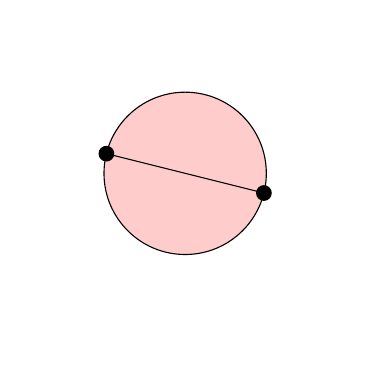
\begin{tikzpicture}
    \clip (-2,2.1) rectangle (2,-2);

    \fill[fill=red!20] (0, 0.25) circle(1.0307764064);
    \draw (0, 0.25) circle(1.0307764064);
    %~ \pattern[pattern color=black!60, pattern=north west lines];


    \fill (-1, 0.5) circle(0.1);
    \fill (1, 0) circle(0.1);
    \draw (1, 0) -- (-1, 0.5);
\end{tikzpicture}
}
        %~ \subfigure{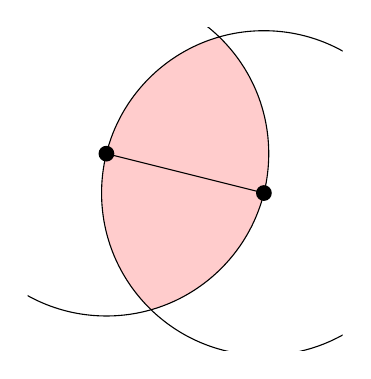
\begin{tikzpicture}
    \clip (-2,2.1) rectangle (2,-2);
    % Shade the intersection where signals collide.
    \begin{scope}
        \clip (-1, 0.5) circle(2.06155281281);
        \fill[fill=red!20] (1, 0) circle(2.06155281281);
    \end{scope}

    \draw (-1, 0.5) circle(2.06155281281);
    \fill (-1, 0.5) circle(0.1);
    \draw (1, 0) circle(2.06155281281);
    \fill (1, 0) circle(0.1);
    \draw (1, 0) -- (-1, 0.5);
\end{tikzpicture}
}
        \subfigure{\tikzset{
    hatch distance/.store in=\hatchdistance,
    hatch distance=10pt,
    hatch thickness/.store in=\hatchthickness,
    hatch thickness=2pt
}

\makeatletter
\pgfdeclarepatternformonly[\hatchdistance,\hatchthickness]{flexible hatch no}
{\pgfqpoint{0pt}{0pt}}
{\pgfqpoint{\hatchdistance}{\hatchdistance}}
{\pgfpoint{\hatchdistance-1pt}{\hatchdistance-1pt}}%
{
    \pgfsetcolor{\tikz@pattern@color}
    \pgfsetlinewidth{\hatchthickness}
    \pgfpathmoveto{\pgfqpoint{0pt}{0pt}}
    \pgfpathlineto{\pgfqpoint{\hatchdistance}{\hatchdistance}}
    \pgfusepath{stroke}
}
\makeatletter
\pgfdeclarepatternformonly[\hatchdistance,\hatchthickness]{flexible hatch nw}
{\pgfqpoint{0pt}{0pt}}
{\pgfqpoint{\hatchdistance}{\hatchdistance}}
{\pgfpoint{\hatchdistance-1pt}{\hatchdistance-1pt}}%
{
    \pgfsetcolor{\tikz@pattern@color}
    \pgfsetlinewidth{\hatchthickness}
    \pgfpathmoveto{\pgfqpoint{0pt}{\hatchdistance}}
    \pgfpathlineto{\pgfqpoint{\hatchdistance}{0pt}}
    \pgfusepath{stroke}
}

\begin{tikzpicture}
    \clip (-2,2.25) rectangle (2,-1.75);

    \begin{scope}
        \clip (-1, 0.5) circle(2.06155281281);
        %~ \fill[fill=blue!20] (1, 0) circle(2.06155281281);
        %~ \draw[pattern=north west lines] (1, 0) circle(2.06155281281);
        \draw[pattern=flexible hatch no,hatch distance=10pt,hatch thickness=0.7pt] (1, 0) circle(2.06155281281);
    \end{scope}

    %~ \fill[fill=white] (0, 0.25) circle(1.0307764064);
    %~ \draw[pattern=north east lines] (0, 0.25) circle(1.0307764064);
    \draw[pattern=flexible hatch nw,hatch distance=10pt,hatch thickness=0.7pt] (0, 0.25) circle(1.0307764064);
    \draw[thick] (0, 0.25) circle(1.0307764064);

    \draw[thick] (-1, 0.5) circle(2.06155281281);
    \fill (-1, 0.5) circle(0.1);
    \draw[thick] (1, 0) circle(2.06155281281);
    \fill (1, 0) circle(0.1);
    \draw[thick] (1, 0) -- (-1, 0.5);
\end{tikzpicture}
}
        \subfigure{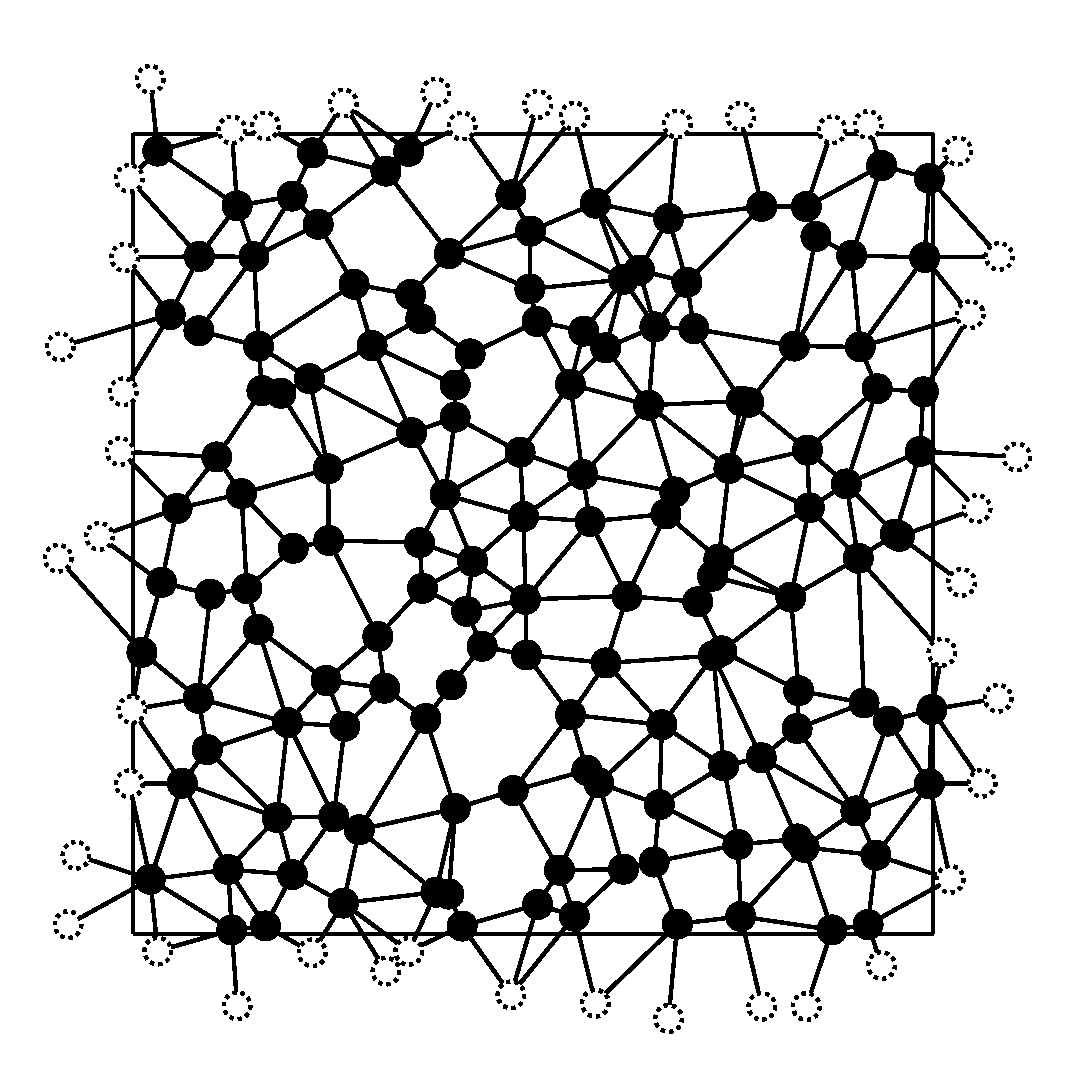
\includegraphics[width=0.3\textwidth]{images/GGL12S03.pdf}}
        \subfigure{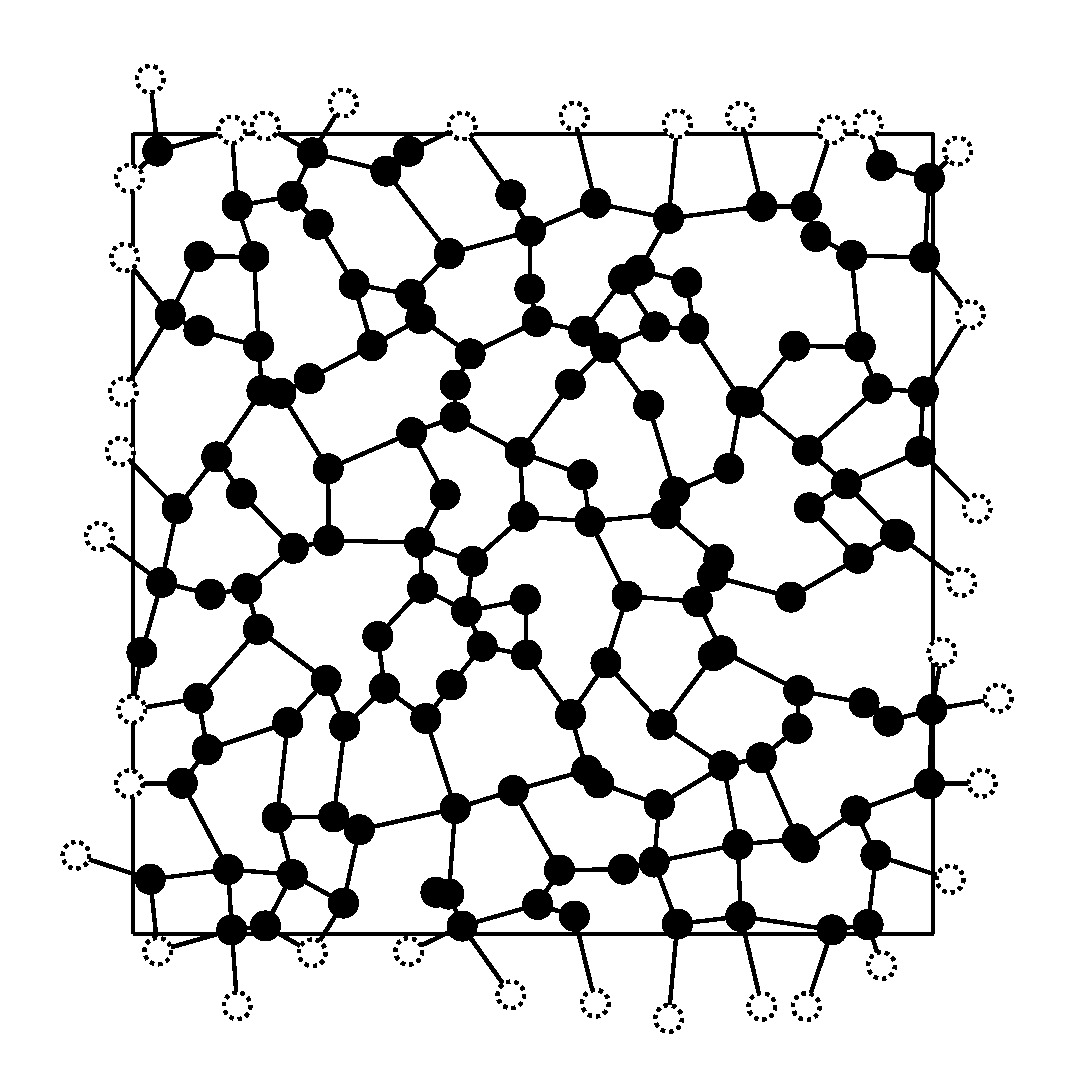
\includegraphics[width=0.3\textwidth]{images/RNGL12S03.pdf}}
        \caption[Definition of the lunes and examples of the Gabriel
                and Relative Neighborhood Graph]
                {Left: Lunes of Gabriel Graph (red) and Relative
                    Neighborhood Graph (blue and red). Middle:
                    Example of a Gabriel Graph. Periodic nodes are
                    dashed. Right: Example of a Relative
                    Neighborhood Graph. Periodic nodes are dashed.}
        \label{fig:lunes}
    \end{figure}

    To construct these graphs the simple way is to test for every
    pair of nodes for every node if it lies in the lune of the pair.
    That is of complexity \(O (n^3)\).\\
    To reduce the complexity one can first create a Delaunay
    Triangulation in complexity \(O (n \log n)\)
    \cite{Leach1992} and test the criterion for each edge, because
    the Delaunay Triangulation is a supergraph of both. But the
    implementation of a Delaunay Triangulation algorithm is not
    trivial and the generation of the graphs is not time critical in
    the scope of this bachelor thesis.\\
    So a tradeoff is to use basicly the simple method but only test
    the criterion for nodes which are near to the lune and abort if
    one node inside the lune is found. To determine which nodes are
    near the lune one can save the position of every node in a
    \emph{cell list} according to \cite{RNGCell} and just test the
    nodes in the cells which resemble a rectangular bounding box of the
    lune.

\subsection{Model}
    The used model is a modified 2D Ising model where the \(N\)sites are
    displaced nodes of a square lattice of edgelength \(L\) with
    periodic boundary conditions. The displacement is randomly gauss
    distributed with the standard deviation \(\sigma\). This \(\sigma\)
    is also called \emph{disturbance paramter} in the following.
    The hamiltonian of the Ising model is
    \(\hat{H} = \sum_{\avg{i,j}}J_{ij}s_{i}s_{j}\)
    where \(\avg{i,j}\) refers to by edges connected nodes.
    The edges are constructed according to the in section
    \ref{sec:graphtypes} defined rules. So that the lattice resembles a
    proximity graph. Each node \(i\) has a spin \(s_i = \pm 1\). Each
    edge has a weight \(J_{ij} = \exp (\alpha (1-d_{ij}))\) with the
    distance \(d_{ij}\) between the nodes \(i\) and \(j\). \(J\) is
    called \emph{interaction}.\\
    For \(\sigma = 0\) this is the standard Ising model with \(J = 1\),
    for which exists an analytical solution \cite{Onsager1944}.\\

    For evaluation the Monte Carlo simulation is is run till the system
    is equilibrated after \(t_{eq}\) sweeps. Then the simulation continues
    and the magnetisation per site \(m\) and energy of the system \(E\)
    are calculated and saved for every \(2\tau\) sweeps. Where \(\tau\)
    denotes the \emph{autocorrelation time} after which two states of
    the system are not correlated anymore.
    For every observable \(O\) the expected value \(\avg{O}\) is averaged
    over different randomly generated lattices \(\overline{\avg{O}}\). The
    errors are estimated by bootstrapping.

\subsection{Critical Temperature $T_c$ and Critical Exponents}
    Because the searched for property -- the critical temperature \(T_c\)
    -- is only defined for infinite systems, hence every computer
    simulation will show some \emph{finte size effects}.
    [vielleicht Bild von intensiver Größe?]
    Despite of this one can obtain \(T_c\) by finite size scaling
    methods \cite[S. ??]{Newman1998} which also yield the critical
    exponents. The critical exponents should not be influenced by the
    disturbance paramter \(\sigma\) [citation needed]. So they will be
    used for consistency cross checking and comparision with the known
    exact values \cite[S. 59]{Pelissetto2002}.\\
    %~ [theorie mit dem Collaps]
    %~ [Erklärung autoscale]
    %~ [Am besten hier direkt die ganze Auswertung rein]
    %~ [weiter ausarbeiten] [sagen, dass man für zwei/drei sigma
    die exponenten reproduziert hat].\\
    Though if one is just interested in the critical Temperature an
    easier approach is to find the intersections of the binder cumulants
    \(g = \brac{3-\frac{\avg{m^4}}{2\avg{m^2}^2}}\) \cite{Binder1981} of different
    system sizes \(L=\sqrt N\).
    Therefore a polynom of degree 4 is fitted to \(g\) in vicinity of
    the intersection. %[vgl. Grafik (villeicht)]
    The arithmetic average of the intersections are plotted [hier schon?]
    %~ [Und den rest der Auswertung]
    \\
